\chapter{Human Factors in using FireflyX}
\label{sec: humanFactors}

Through our user study, we performed analysis on both qualitative and quantitative data. These qualitative data include participant utterances during think out aloud protocol, coded observations during usability tests, comments submitted with test instruments and others. These qualitative data were analyzed with the quantitative data in order to be able to bridge findings and statistics. Quantitative data includes AttrakDiff scores, time it took to complete tasks, expert rating scores, and other measures. 

\subsection{Behavioral Findings}

We were able to observe findings that describe how children behave and act while using our mobile application. These behaviors go from subtle cues all the way to mannerisms that are obvious during the usability tests.

\textit{Nodding of head while listening to firefly.} We were able to observe that certain participants listen and move with the sound output of the firefly models in the mobile app. P1, P2 and P3 were the most obvious in demonstrating these traits.  They began by listening to the tune and then nodding or moving their heads along in sync with the tune as they listen to the sound output. This happened while they were trying to verify the fireflies that they have created. We then believe that this nodding behavior aids in memory as first introduced by \citeA{de2018optimizing} where the researcher also mentioned that a child nodding his head confirms a “yes” showing a positive kind of response.

\begin{figure}[H]
    \centering
    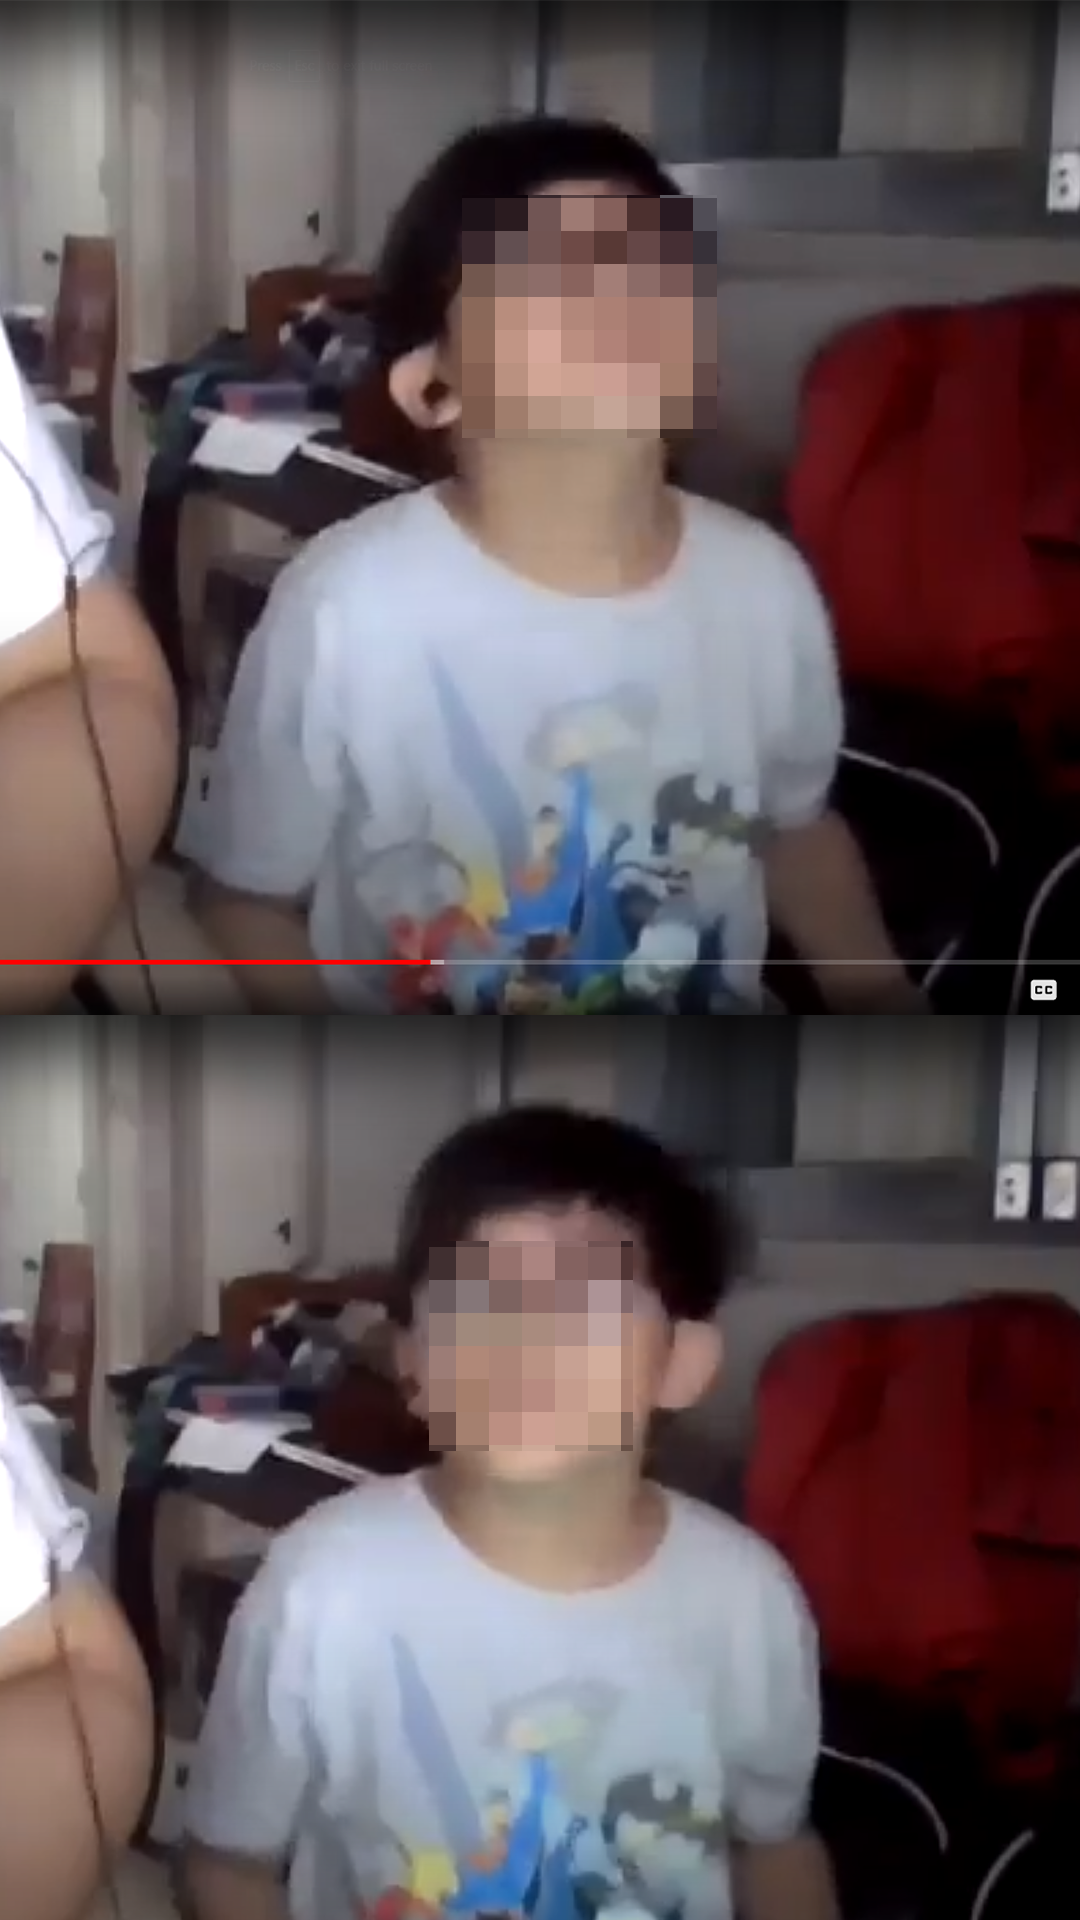
\includegraphics[width=8cm]{figures/Results/UTpictures/noddingboyblur.png}
    \caption{Participant nodding head while listening to playback}
    \label{fig:noddingparticipant}
\end{figure}

In Figure \ref{fig:noddingparticipant}, we can see that the the participant is nodding his head as he listens to the playback of the iPad.

\textit{Eagerness, playfulness and confidence.} In using FireflyX, we observed that 4 out of 5 participants (P1, P2, P4, and P5) would tend to tap the tablet and nearby surfaces more frequently. They would \textit{overtap} (when they are supposed to tap an element once, but instead would tap it more times that they are supposed to). This appears to be like a display of eager behavior towards exploring the application more. We believe that this is due to the sandbox nature of the application which encourages playful behaviour. This gives the children the feeling as if they were immersed in an actual sandbox while using the application \cite{inal2007flow}. The participants also exhibited elevated or increased levels of happiness as seen in their energetic display when they confirm that they did their tasks correctly.  Whenever they would listen to their outputs and hear that it matches the expected output, they tend to clap and exhibit energetic behavior out of sheer excitement. The participants also showed to have an improved mood (which means it is a positive feeling) when they receive feedback on their tasks (that they did it right). Notably, P4 exhibited laughter even when they committed technical mistakes (e.g. notes are off-pitch) during their tasks. We believe that accomplishing tasks can help uplift the mood of the child and give them a boost in their morale. The study by \citeA{elahi2017xylotism} also mentioned that when the child feels validated and is reassured, they feel more motivated to use the application. They also begin to show signs of increased confidence the longer they use the FireflyX. Comments like "ez [easy]" and moments when participants asserted that they are finished with the task (even if they are only being asked) were observed as they use the application. We believe that children become more confident in using the application if they spend more time using it. As \citeA{frokjaer2000measuring} states, the time spent in using a system indicates that there is learning, and this will eventually enable them to learn to do their tasks more efficiently. Our data supports this as we observed a moderate positive correlation as seen in Table \ref{C3} with the scores and the time of tasks 4 and 5 \textit{(r-val = 0.5)}. Indicating that as the participants take their time (averaging 1444.2 and 1123.4 seconds respectively) in completing the task the higher rating (averaging a score of 23.7 and 21.2 over 28 respectively) they get from the music experts. We chose task 4 and task 5 because this is the stage where they are encouraged to play around and explore with the application with minimal guidance in order to finish the task.

\begin{figure}[H]
    \centering
    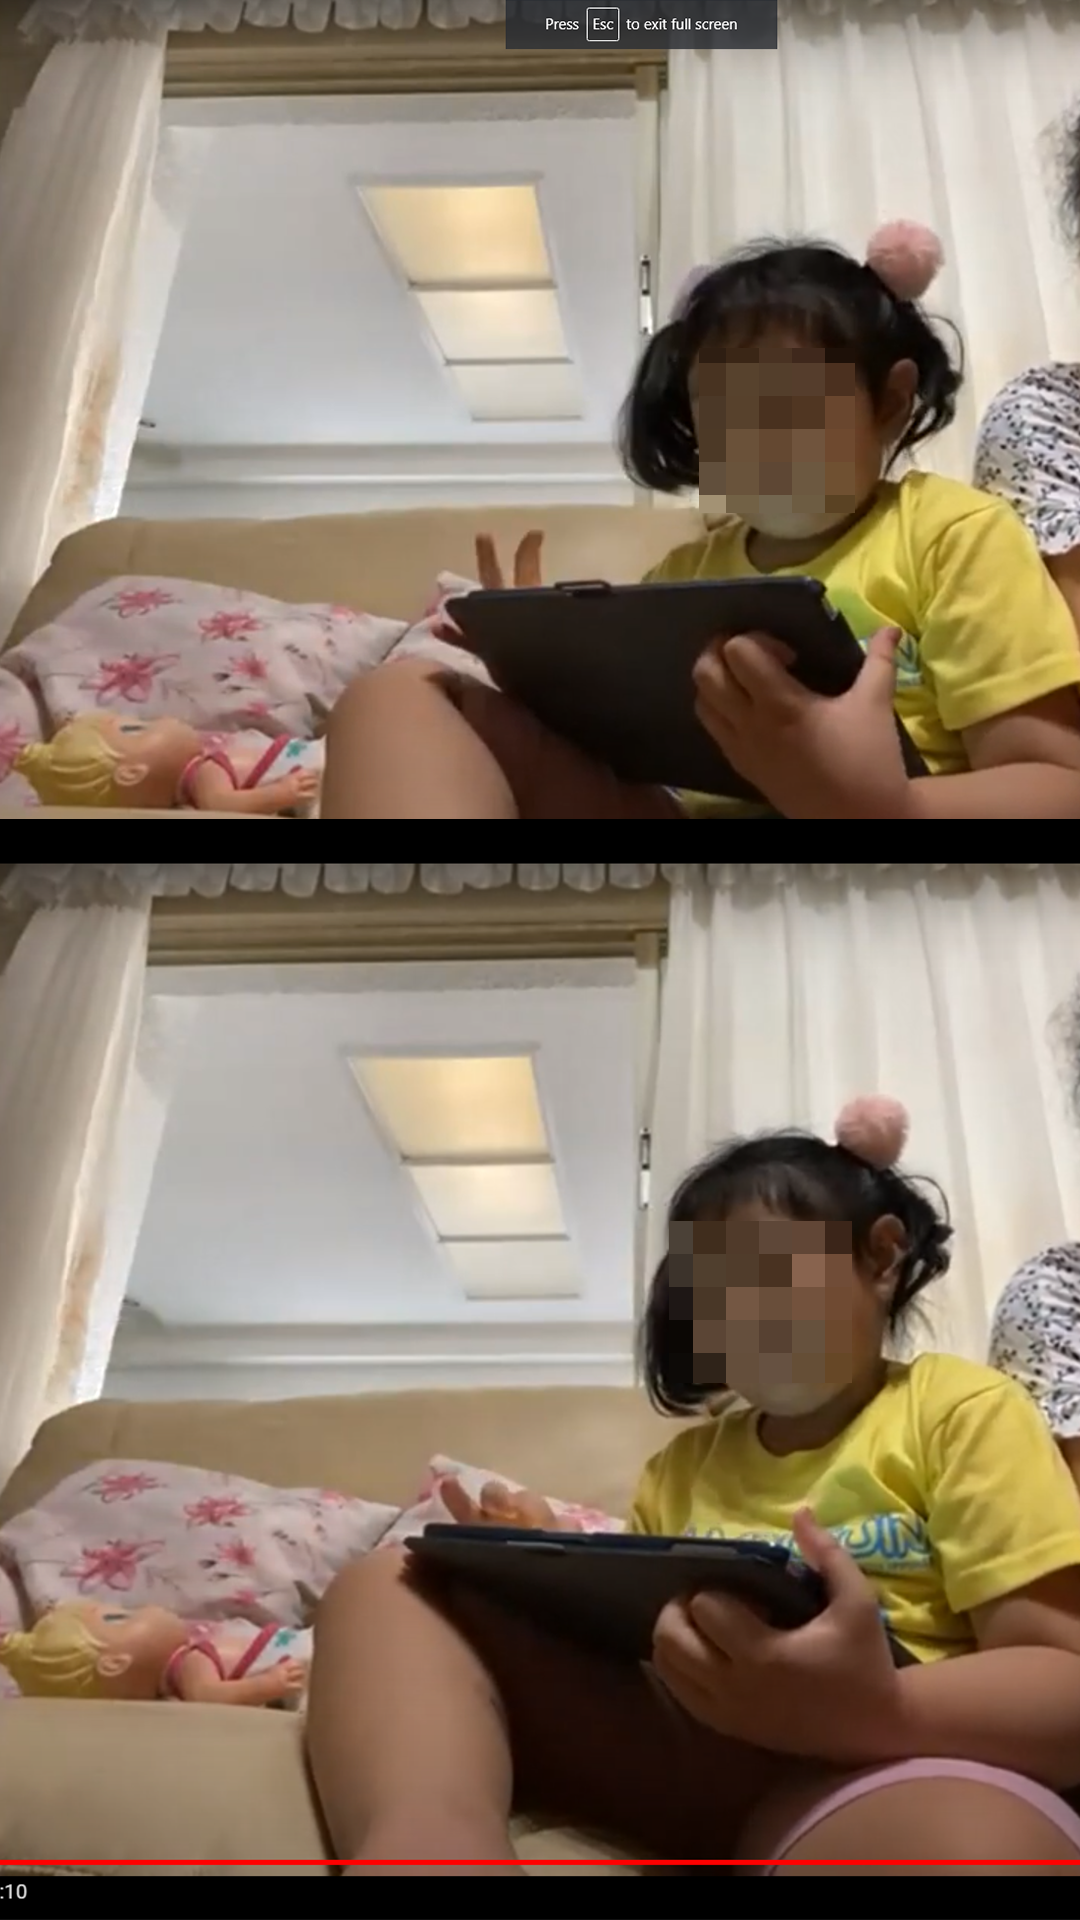
\includegraphics[width=8cm]{figures/Results/UTpictures/Tapping.png}
    \caption{Participant tapping the back of an iPad}
    \label{fig:tappingparticipant}
\end{figure}
\begin{figure}[H]
    \centering
    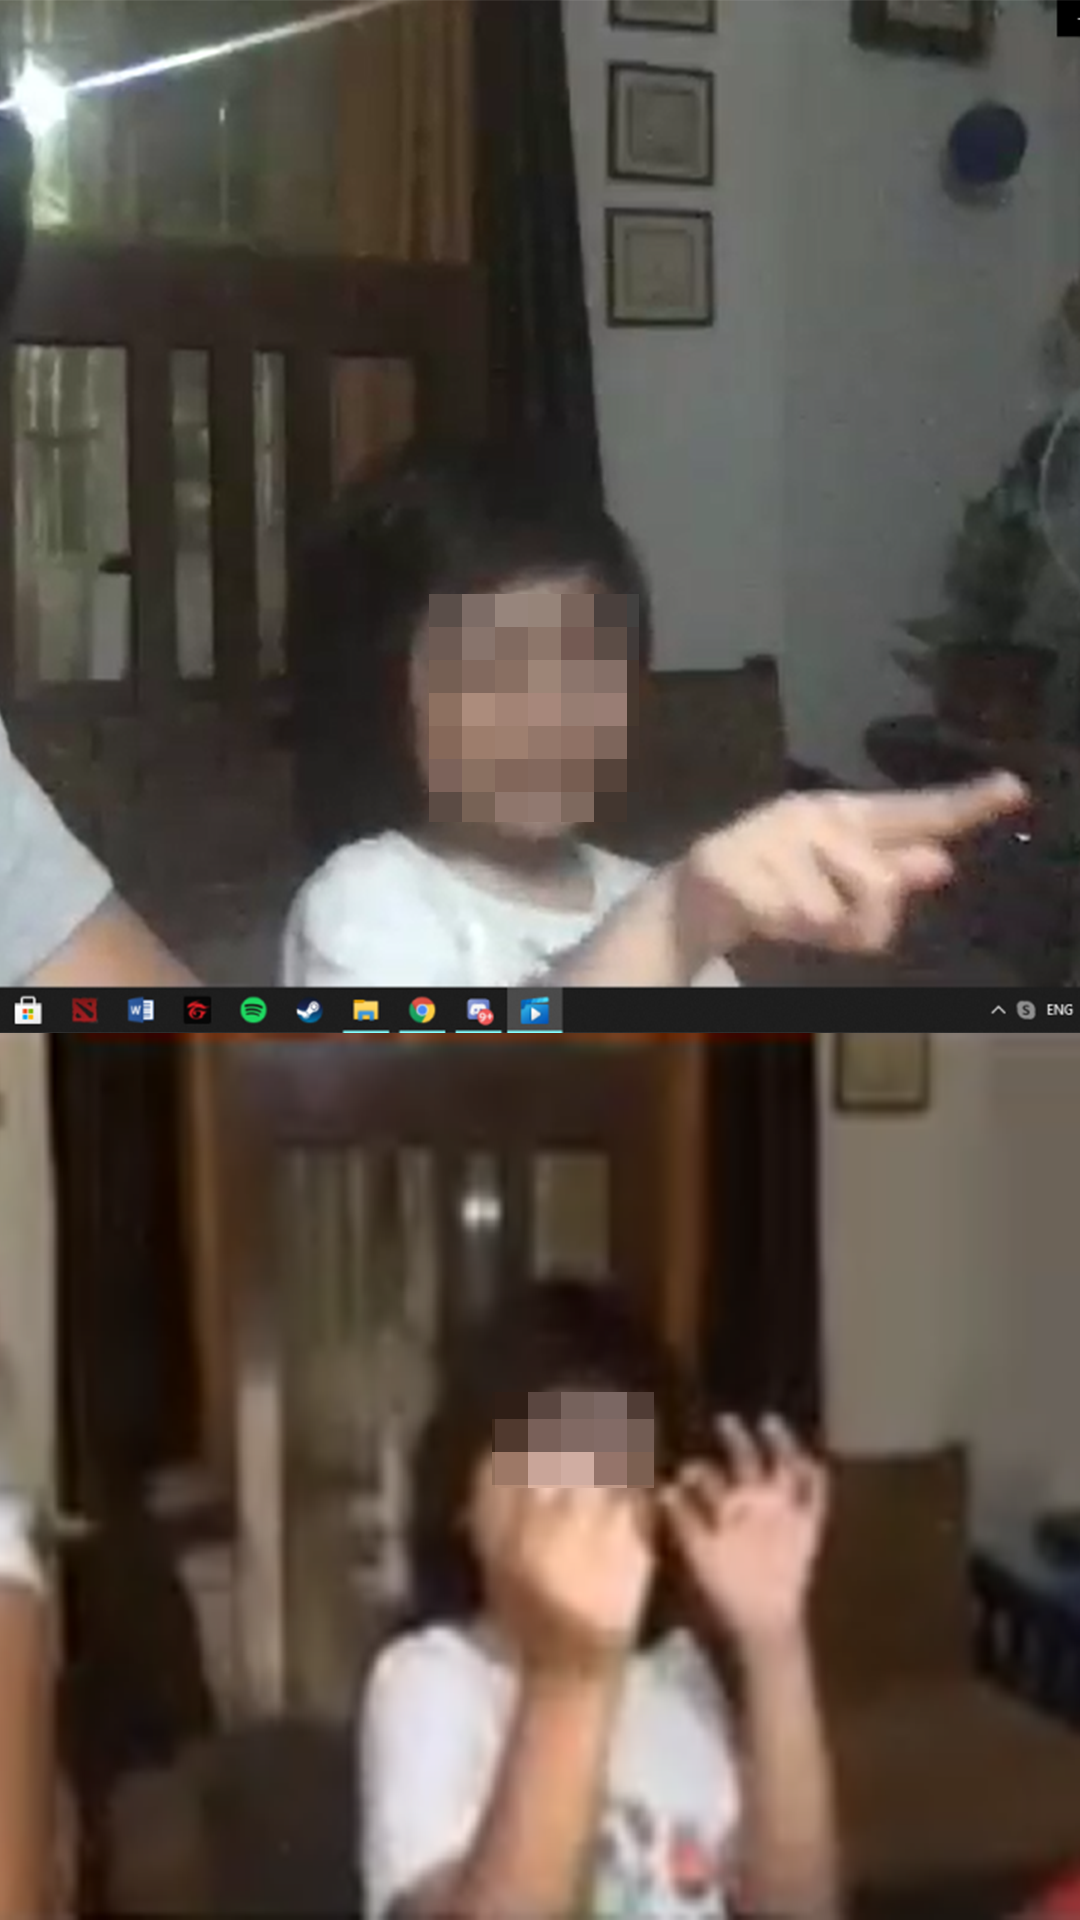
\includegraphics[width=8cm]{figures/Results/UTpictures/fingerplaying.png}
    \caption{Participant playing with fingers}
    \label{fig:fingeringparticipant}
\end{figure}

In Figure \ref{fig:tappingparticipant}, we can see that the the participant is playfully tapping and fidgeting the back of the iPad while doing the task. Same as Figure \ref{fig:fingeringparticipant}, the participant is also playing with their fingers while using the application.

\textit{Annoyance, committing mistakes and seeking validation}. We also observed that some participants are more easily-annoyed and become more scared than others. These were more commonly-observed from P1 and P2 when they are trying to complete their tasks and commit mistakes along the way. They get frustrated and annoyed when making mistakes or when they do not figure out what is wrong with what they are doing.  These were more common while they were doing tasks 4 and 5. This can be verified in the results of the Attrakdiff survey. The word pair \textit{Undemanding-Challenging} leaned more towards challenging (HQ-S: 5-7 points). We believe this is because tasks 4 and 5 were designed to be more difficult than the other tasks (which are more exploratory in nature). These were further observed in specific instances where they said \textit{"is there a time limit?"}, and \textit{"I am not sure"}. These comments describe as if the participants were afraid to commit mistakes and are conscious of their output. We believe that children are afraid committing mistakes, as seen as well in the study by \cite{hourcade2015child}. Their work integrated the social aspect of committing mistakes and doing tasks in familiar scenarios. Children tend to copy how adults act and sometimes would do things similar to the way they see from their guardians. While the children would only notice how the adults would successfully do their tasks, they would not notice the mistakes made along the way as they might not realize or know that was wrong. Participants P3 and P4 were observed to constantly refer to their guardian as they progress through their tasks. They do this to check if they are on track which can be interpreted as a social behavior that seeks validation. In the Figure \ref{fig:allassistance}, we observed a strong negative correlation as seen in Table \ref{C1} \ with the number of times they referred to their guardians for help and to their respective age \textit{(r-val = -0.9)}. Indicating that as the participants age decrease they would tend to ask for more assistance from their guardian.

%in the previous chapter it shows that the two were more reliant on their parents in getting the correct answer.

\subsection{Attention Findings}
We observed specific behaviors that describe how children pay attention when using FireflyX. These findings can describe how the thinking out loud and visual elements help them in learning music.


\textit{Retaining memory by thinking out loud}. We observed that there was a difference in how the participants made use of the available reference while they do their tasks. P1 and P4 were more reliant to the candy diagrams (as supplementary materials to help them read the music sheets) as compared to P2, P3, and P5. In Task 4, the candy diagrams were intentionally replaced with actual music sheets. P1 and P4 made obvious reactions to this subtle change. The other participants (P2, P3 and P5) showed that they were fine with using them. Based on their demographic information as seen in Table \ref{tab:ParticipantDemographic}, P2, P3, and P5 were more knowledgeable in music compared to the other participants. We also noticed that these 3 participants used the music sheets more confidently and were exhibiting the thinking out loud protocol more. We believe that this aids in memorability as previously-studied by \citeA{gagne1962study}. They found that there is a memory advantage in thinking out loud or saying the words compared to keeping it to yourself in your head. Interestingly, P2, P3, and P5 had a mean average of x̅ = 6.3 for their rating in memory while P1 and P4 had mean average of x̅ = 4.6 which supports the idea that thinking out loud helps with retaining information.

\textit{Convenient visual matching through playful cues}. One important finding that strengthens the design of our application was observed when we got comments pertaining to the visual elements of the application that participants liked. The children were able to easily-connect the firefly model and their corresponding musical rudiments. The participants were also able to easily-grasp the concept represented by the candy diagrams. These can be seen in the results of the Attrakdiff tests.  The scores were leaning towards the Stylish, Creative and Appealing criteria based on the hedonistic qualities in the form (HQ-S and ATT scores were between 5 and 7). This indicates that the participants really liked the how the visual elements are portrayed and how it helped them understand the musical rudiments. The design helped in attracting and motivating the children to keep using the application. This was also seen in the studies by \cite{cohen2011young,burton2016music,chung2017designing} which all explicitly mentioned the importance of having a child-friendly design helps children become motivated in using the app. This also helped catch and maintain their attention which helped them in having an increased pace in learning. 

\subsection{Learning Findings}
We observed specific behaviors that describe how children learned and used FireflyX. These findings can describe their attitude and preference towards learning and difficult content. 

\textit{An accessible visual reference to aid music learning}. We developed and deployed a project website\footnote{https://comet.dlsu.edu.ph/FireflyX/} to serve as an all around guide for participants and experts. However, the website seemed to be of more use in the completion of their tasks, than what was originally-intended. All participants used the website during the majority of their tasks. They used the site to refer to the patterns that they wish to copy from it.  Interestingly, P2 and P3 were relying less on the site as they were more used to the application (mention their higher score from expert once the evaluation forms is finalized). Having a guide were able to help the participants learn the application and the concepts sooner \cite{pashler2007organizing}. Making the guides clearer and arranging them in an organized way helps stimulate learning thereby making it easier for them to copy; little by little getting used to learning a particular topic. With the help of the guide, they learned to use the application and started memorizing the notes that corresponds to the candies. All participants were observed to have improved in remembering what the buttons do, and in turn, they navigated through the application faster as the sessions go by. We believe that if children get used to a specific layout and the more time they spend using it, they instinctively press the buttons that they need given the task \cite{wiedenbeck1999use, ibharim2014ibuat}. These studies mention that when the elements are designed well and are understandable by the child in a glance, they will tend to learn to use the application faster.

\textit{Ignoring their obvious mistakes.} Some participants tend to deliberately ignore their mistakes while they validate their output through the audio playback feature. Even after they preview a specific sound or tone and notice that there was an obvious error, they still decided to push with that firefly configuration. We believe that this is because some participants may want to finish the task for the sake of finishing. This was very prevalent in Task 5 which intentionally was a difficult challenge to begin with. The completion times for T5 averaged 1073.75 seconds and the expert ratings were around  21.2/28. We observed a strong positive correlation as seen in Table \ref{C2} \with the time spent in task 5 and their scores  \textit{(r-val = 0.8)}. Indicating that as the participants spend more time in doing task 5 their scores tend to increase.

\textit{Findings on Handedness.} Four (4) participants were recorded to be right-handed. Interestingly, 2 of these right-handed participants (namely P3, P4) used their non-dominant hand (left) in performing majority of their tasks. This is not the case for P1 and P5, who are right-handed and also used their dominant hand for their tasks. For the case of P4 (RH, M, 7), this was because of the current test setup where his tablet was placed on the left side of the laptop. He used his left hand more in performing his tasks, while he used his right hand to operate the laptop (in order to specifically look at the pitch and rhythms in the site). P3 (RH, F, 6) showed cross-handedness (formerly called mixed-handedness in the literature) in performing the tasks. She would switch between hands to select element in the screen depending on which was closer to that hand. The sole left-handed participant, P2 (M, 8) demonstrated behaviour similar to that of P3. He was mixed-handed as well like P3.

\textit{Unsupervised learning vs intended guided learning for children}. Participants exhibited trial and error as they used the application. As they made more trials and revisions, they tend to re-calibrate and fine-tune the pitches and patterns they compose with the fireflies. They repeatedly did this until they were somewhat satisfied with their work. This was observed across all five (5) participants and all their tasks especially on tasks 3 and 4. With regards to task 5, even though participants ignored their mistakes as stated in the previous section, they still managed to explore until they actually grew tired of their tasks. This allowed the children to reflect their own mistakes without being given the answer by the application (unsupervised). As we are using a sandbox environment, this enabled the participants to explore several possible outcomes until they produce a relatively-satisfying output.